\hspace{1.5cm}
A aquisição das imagens se deu junto ao catalogo do Instituto Nacional de Pesquisa Espacial (INPE). Foram adquirido imagens do LAndsat 5, respectivamente 1999 e 2011, da cidade de Manaus-AM. A figura \ref{Aquisição1}, mostra o processo de escolha da região de interesse. Neste caso foi escolhido a região da cidade de Manaus-AM.\\
\begin{figure}[!htpb]
        \centering
        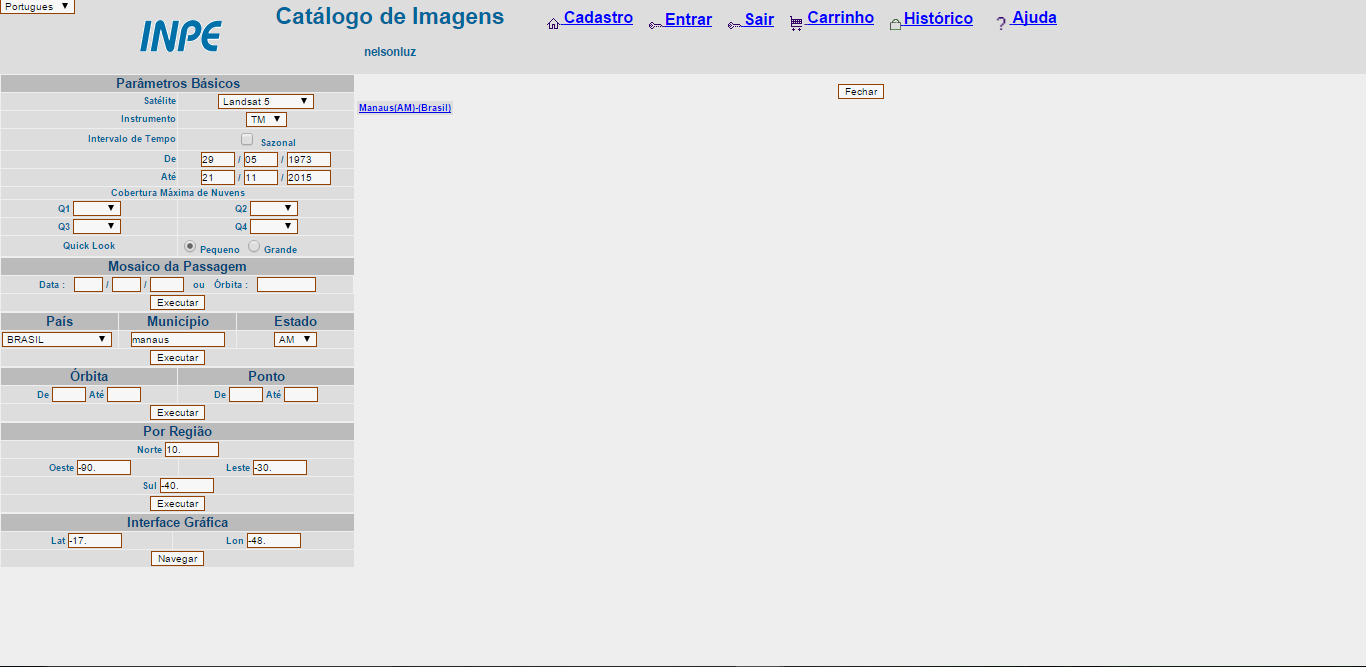
\includegraphics[scale=0.3]{imagens/aquisicao.png}
        \caption{site do INPE - Escolha da área de interesse.}
        \label{Aquisição1}
\end{figure}

\hspace{1.5cm}
Após a definição da área de estudo é necessário a seleção,figura \ref{Aquisição2}, da posição do satélite que melhor totalize a região estudada. As imagens da posição 231 melhor atendeu aos interesse, pois se tinha uma visão do todo da cidade.\\
\begin{figure}[!htp]
        \centering
        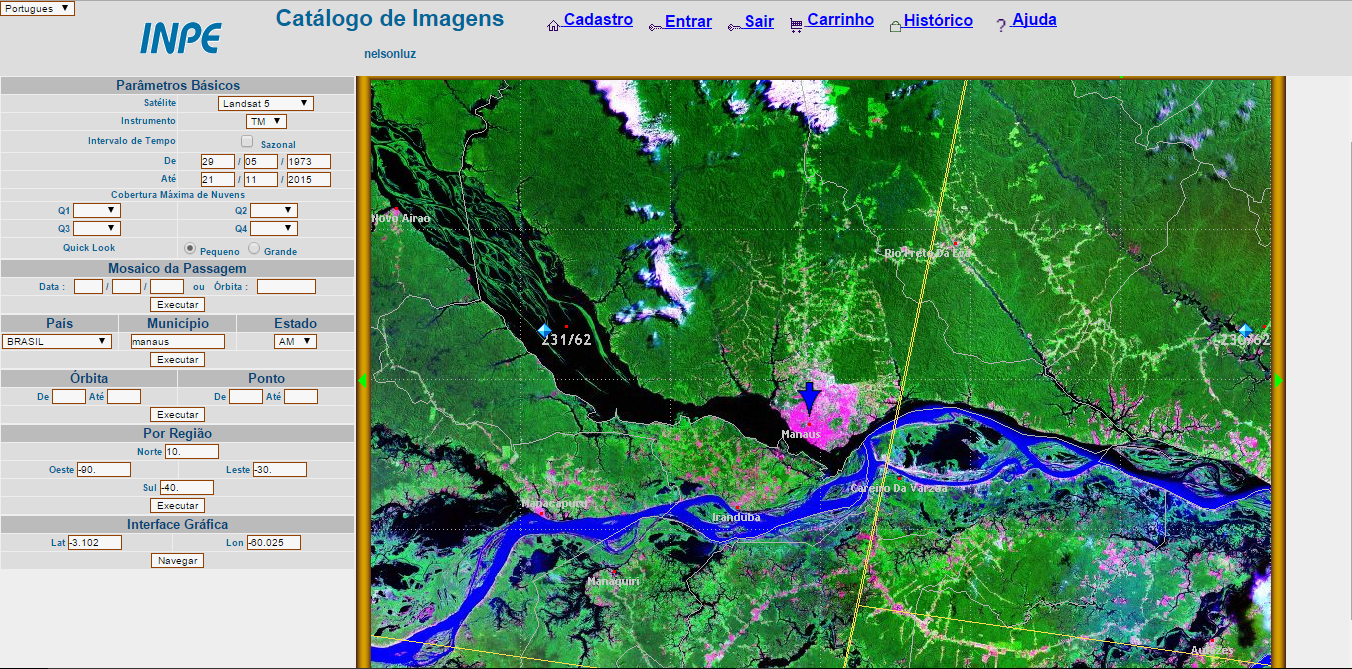
\includegraphics[scale=0.3]{imagens/aquisicao_02.png}
        \caption{site do INPE - Seleção da posição da imagens.}
        \label{Aquisição2}
\end{figure}

\hspace{1.5cm}
O INPE disponibiliza uma vasta coleção de imagens, do Landsat 5, compreendendo o período de 1984 a 2011. Dentro do seu catalogo, figura \ref{Aquisição3}, selecionamos e colocamos no carrinho as imagens que irá atender, nos seus respectivos anos. Foram selecionado os anos de 1999 e 2011, para se obter analise temporal de mais de 10 (dez) anos. \\
\begin{figure}[!htpb]
        \centering
        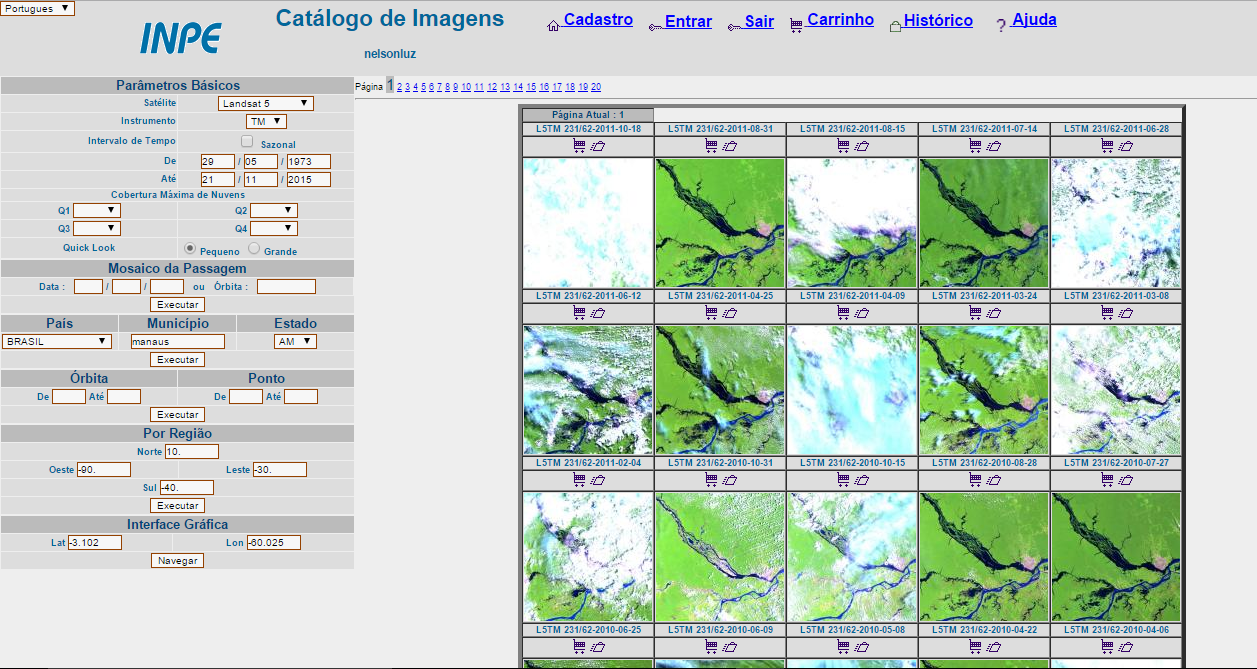
\includegraphics[scale=0.3]{imagens/aquisicao_03.png}
        \caption{site do INPE - Colocação das imagens selecionadas no carrinho.}
        \label{Aquisição3}
\end{figure}
\hspace{1.5cm}
As Imagens selecionadas são disponibilizadas através de um link "ftp", disponibilizado pelo INPE e enviado ao email do usuário cadastro no sistema.